\chapter{Projekt aplikacji}
	% uml-e, mvc. wzorce projektowe, może maven i javaDoc????????
	
	\section{Podział aplikacji}
	Aplikację podzielono na 3 mniejsze moduły, xbit, z80emu-core oraz z80emu-gui z czego każdy z nich jest osobnym mniejszym projektem, który używa narzędzia ,,Maven" do zautomatyzowania procesu budowy oprogramowania. Ich pliki jar są przetrzymywane w platformie mymavenrepo.com jako prywatne repozytorium, zabezpieczone hasłem przy pomocy funkcji protokołu http "basic auth". Każdy z projektów może zostać wysłany do zdalnego serwera za pomocą komendy ,,mvn deploy:deploy". Komenda ta przeprowadza testy jednostkowe, kompiluje kod javy do kodu bajtowego JVM, dodaje zewnętrzne bliblioteki jar i umieszcza plik wykonywalny na serwerze.
	
	Aby umożliwić integracje z serwisem mymavenrepo.com pliki pom.xml zawierają wpisy zaprezentowane w fragmencie kodu \ref{listing:myMavenRepoPom}. Ponieważ repozytoria maven są ustawione jako prywatne, należy odnaleźć w systemie plik ~/.m2/settings.xml podać w nim dane pozwalające na autoryzacje za pomocą "http basic auth". Przykład konfiguracji przedstawiono w kodzie \ref{listing:myMavenRepoSettings}
	
	\begin{listing}[h]
		\inputminted{xml}{listings/myMavenRepoPom.xml}
		\caption{fragment pliku pom.xml umożliwający integracje z serwisem myMavenRepo}
		\label{listing:myMavenRepoPom}
	\end{listing}

	\begin{listing}[h]
		\inputminted{xml}{listings/myMavenRepoSettings.xml}
		\caption{fragment pliku settings.xml przechowującego dane utoryzacyjne do serwera myMavenRepo}
		\label{listing:myMavenRepoSettings}
	\end{listing}

	Przetrzymywanie plików wykonywalnych w zewnętrznym serwisie ułatwia zarządzanie wszystkimi trzema projektami, pozwala na ich wersjonowanie, i łatwiejsze budowanie aplikacji. 

	\section{XBit}
	Java jest językiem programowania wysokiego poziomu, kompilowanym do kodu bajtowego. Z tego powodu nie jest on zazwyczaj stosowany w emulacji, gdyż kod emulatora musi być uruchamiany w maszynie wirtualnej, co nie należy do optymalnych rozwiązań.
	
	Innym poważnym problemem Javy jest brak typów danych przechowujących tylko wartości dodatnie. James Gosling, jeden z twórców Javy tak argumentuje ich brak: 
	,,Dla mnie jako projektant języków programowania, do których tak naprawdę ostatnimi czasy się nie zaliczam, coś prostego oznaczało skończenie na założeniu że losowy deweloper będzie w stanie zapamiętać specyfikacje. 
	Ta definicja mówi, że na przykład Java i wiele innych języków nie są proste, i w rzeczywistości wiele języków kończy z funkcjonalnościami których do końca nikt nie rozumie. Spytaj jakiegoś programistę języka C o dodatnie typy liczbowe, i odkryjesz że prawie żaden programista C faktycznie nie rozumie co dzieje się z typami bez znaku, czym jest arytmetyka liczb całkowitych. Takie rzeczy sprawiły że C jest językiem skomplikowanym. Myślę że w tej kwestii Java jest prosta"\cite{javaGoslingInterview}.
	
	Problem ten rozwiązano tworząc własną bibliotekę o roboczej nazwie XBit. Przechowuje ona liczby 8 i 16 bitowe, które mogą być interpretowane zarówno jako wartości całkowite jak i liczby w kodzie uzupełnień do dwóch. Biblioteka potrafi zwrócić konkretne bity, stworzyć reprezentacje liczby z pojedynczych bitów i typów prymitywnych, obudowuje operacje arytmetyczne z uwzględnieniem przepełnienia i przeniesienia. Kod projektu z jej użyciem staje się czytelniejszy i łatwiejszy do ewentualnej refaktoryzacji. 
	
	Bibliotekę zaprojektowano w taki sposób aby była możliwie jak najbardziej uniwersalna, i można ją było użyć nie tylko podczas emulacji Zilog-a Z80. ale także innych procesorów. 
	
	\subsection{Możliwości}
	Za cel obrano następujące funkcje:
	\begin{itemize}  
		\item odwzorowanie liczb 8 i 16 bitowych
		\item możliwość stworzenia reprezentacji liczb 8 i 16 bitowych z typów prymitywnych 
		\item interpretacja liczb w naturalnym kodzie binarnym lub dopełnień do dwóch
		\item operacje na pojedynczych bitach(możliwość zmiany, odczytu bitu o danym indeksie)
		\item opcja odczytania grupy bitów (odczytanie kilku bitów podając indeks pierwszego i ostatniego bitu)
		\item interpretacja liczb 16 bitowych w formacie big endian lub little endian
		\item operacje arytmetyczne (dodawanie, odejmowanie)
		\item operacje bitowe na liczbach (negacja, alternatywa, koniunkcja, przesunięcia bitowe)
		\item uwzględnienie przy operacjach arytmetycznych przepełnienia oraz przeniesienia
	\end{itemize} 
	
	\subsection{Założenia projektowe xBit}
	Przed przystąpieniem do implementacji rozwiązania, zaprojektowano publiczny interfejs biblioteki w języku uml, zaprezentowany na grafice \ref{img:xbitUml}. Ustalono także założenia projektowe które zaprezentowano poniżej. 
	
	\begin{figure}[h]
		\centering
		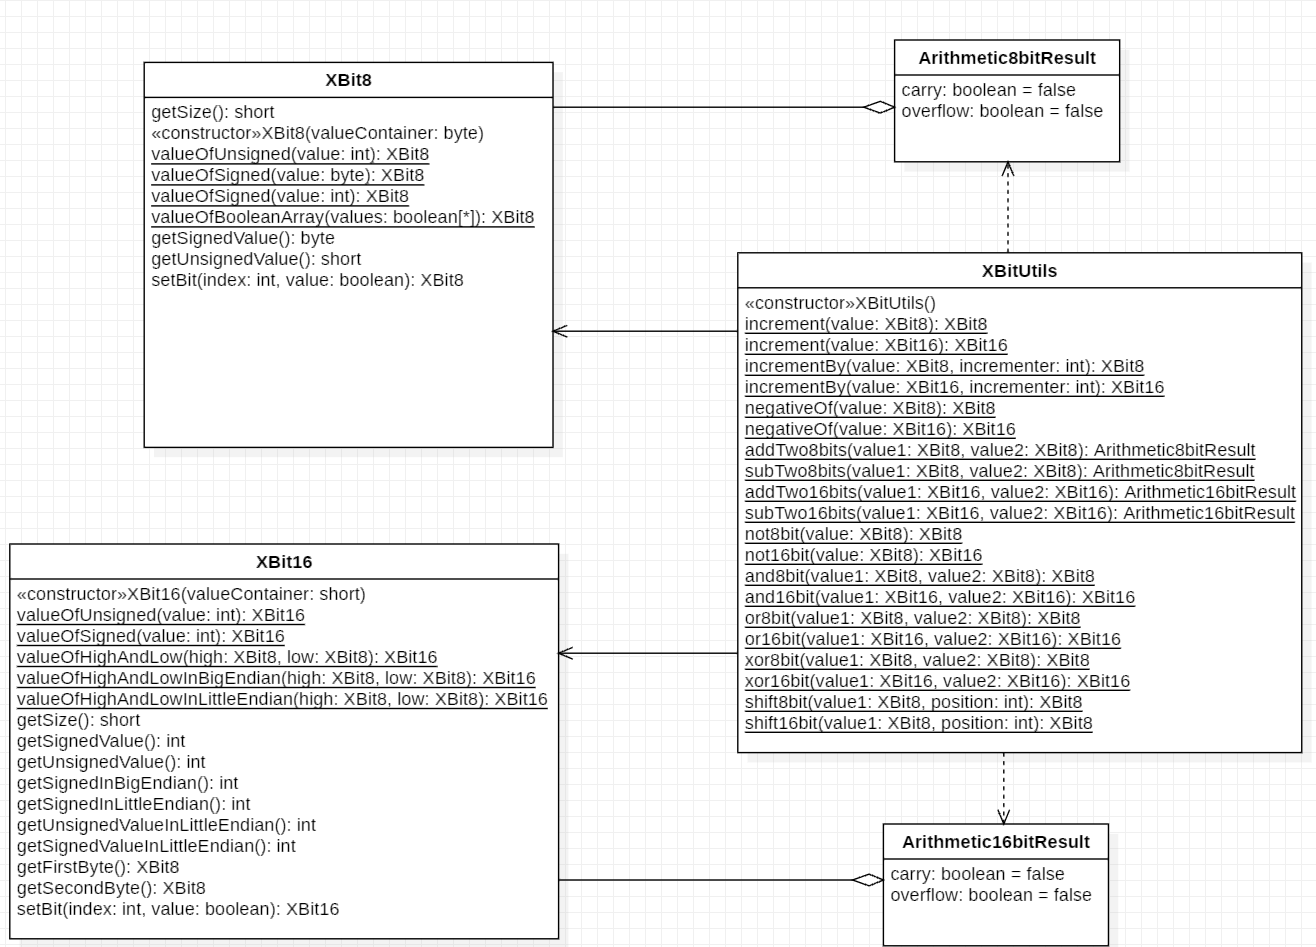
\includegraphics[width=1\textwidth]{xbitUml}
		\caption{projekt uml biblioteki xbit}
		\label{img:xbitUml}
	\end{figure}
	
	\subsubsection{Klasy XBit8 i XBit16}
	Klasy XBit8 oraz XBit16 to reprezentacje liczb 8 i 16 bitowych. Postanowiono, że nie będą one w stanie zmienić swojej wewnętrznej wartości, swego stanu (z angielskiego nazwano by je "immutable"), tak jak obiektowe reprezentacje typów prostych w javie (Short, Long, Integer itp).  Przez podjęcie tej decyzji projektowej, metody które powinny zmienić stan obiektu, klonują istniejący obiekt a następnie modyfikują odpowiednio jego stan. Przykładem takiej metody jest setBit(index: int, value: boolean) klasy Xbit8 oraz Xbit16. Funkcja ta nie zmienia bitu obiektu na rzecz którego została wykonana, a jedynie zwraca kopie obiektu, z zmodyfikowanym odpowiednim bitem. 
	
	Zalety zastosowania obiektów niezmiennych:
	\begin{itemize} 
		\item Prosta implementacja oraz łatwe debugowanie kodu.
		\item Garbage Collector jest zoptymalizowany pod względem pracy z tego typu obiektami.   
		\item Łatwość zapisywania obiektów do pliku lub pamięci podręcznej (z ang. cache).
		\item Bezpieczne używanie obiektów niezmiennych w programach wielowątkowych, co umożliwiałoby emulacje potokowości CPU. Jeden wątek w takim przypadku mógłby być odpowiedzialny za jeden stopień potoku, np osobny wątek pobierał by instrukcje z pamięci, inny dekodował instrukcję, kolejny wykonywał i tak dalej.
		\item Możliwość użycia obiektu jako klucz, np w HashMap. 
	\end{itemize}
	
	Wadą zastosowania obiektów niezmiennych jest optymalizacja, i zwiększone użycie pamięci, co mimo wszystko nie powinno być przeszkodą dla współczesnych komputerów. Ze względu na przewagę zalet w stosunku do jednej wady postanowiono użyć obiektów niezmiennych w bibliotece.
	
	\subsubsection{Klasa XBitUtils, Arithmetic8bitResult, Arithmetic16bitResult}
	Klasa XBitUtils jest odpowiedzialna za wszystkie operacje arytmetyczne oraz bitowe. Większość z jej metod zwraca obiekty klas XBit8 lub XBit16. Wyjątkami są metody wykonujące dodawanie lub odejmowanie, które oprócz zwrócenia wyniku operacji powinny informować o wystąpieniu przeniesienia lub przepełnienia. Z tego zaprojektowano  klasy Arithmetic8bitResult oraz Arithmetic16bitResult które zawierają następujące pola:
	\begin{itemize}
		\item obiekt klasy XBit8 lub XBit16 będący rezultatem operacji
		\item dwie zmienne typu boolean informujące o wystąpieniu przeniesienia i przepełnienia
	\end{itemize}
		
	
	
	\section{z80emu-core}
	Z80emu-core to moduł mający za zadanie wykonywać emulację oraz udostępniać zestaw metod umożliwiający  manipulacje tym procesem. Za cel obrano stworzenie takiego interfejsu, który pozwalał by na użycie Z80emu-core w innych projektach, które emulują urządzenia zbudowane między innymi z Ziloga Z80. Jako przykład można podać emulator przenośnej konsoli Game Boy firmy Nintendo z 1989 roku która jako główny procesor używała Ziloga Z80. 

	Za cel obrałem implementacje następujących funkcji:
	\begin{itemize}  
		\item możliwość wykonania wszystkich 158 instrukcji procesora
		\item zestaw metod umożliwiających zmianę stanów rejestrów
		\item emulacja zewnętrznej pamięci
		\item możliwość podłączenia urządzeń wejścia/wyjścia
		\item wywołanie przerwania maskowanego oraz niemaskowanego (Z80 posiada dwa rodzaje przerwań)
	\end{itemize}
	
	\subsection{Publiczny interfejs modułu z80emu-core}
	Publiczny zestaw metod służący manipulacją samym procesem emulacji jak i urządzeniem pokazano na grafice \ref{img:z80emuCoreUml}. Cała mechanika działania modułu została ukryta w trzech klasach: Z80, RegistersBank i DuplicableRegisterSet. 
	
	Klasa Z80 zawiera zestaw funkcji manipulującymi samą emulacją, oraz wartościami liczników i mniejszych rejestrów procesora. Niżej opisuje najważniejsze z nich:
	\begin{itemize}  
		\item Z80(memory: Memory, ioDevice: IoDevice) - konstruktor, przyjmujący dwa parametry wymagane do poprawnego działania. Parametr ,,memory" oraz "ioDevice to obiekty implementujące interfejsy o tych samych nazwach. Reprezentują one kolejno moduł pamięci oraz urządzenia wejścia wyjścia podłączone do procesora. Użytkownik używający modułu Z80emu-core ma powinien samemu zaimplementować ich działanie, z zależności od otoczenia w jakim chce emulować urządzenie. 
		
		\item runOneInstruction() - metoda wykonująca jedną instrukcję procesora, za jej pomocą wykonane zostanie pobieranie, dekodowanie, wykonywanie rozkazu, ale również obsługa przerwań, inkrementacja liczników.
		
		\item makeInterupt(addressBus: XBit8), makeNonMaskableInterupt(addressBus: XBit8) - metody powinny zostać wywołane między kolejnymi wywołaniami runOneInstruction(). Ich zadaniem jest zgłaszanie przerwań. Parametr addressBus to wartość jaka została by ustalona na magistrali danych podczas przerwania, gdyby zostało ono wykonane w prawdziwym urządzeniu.
	\end{itemize}
	
	Wartym przypomnienia jest, że Zilog Z80 jest procesorem posiadającym dwa zestawy rejestrów ogólnego przeznaczenia (do nich należąc rejestry A,B,C,D,E,H,L,F oraz ich 16bitowe odpowiedniki). Takie rozwiązanie jest optymalne, w przypadku gdy procesor często wykonuje obsługę przerwań. W klasycznym podejściu, podczas przerwania zestawi rejestrów ogólnego przeznaczenia zapisany zostałby na stosie, co jest czasochłonną operacją. Projektanci Ziloga Z80 postanowili stworzyć drugi alternatywny zestaw rejestrów ogólnego przeznaczenia, który zostaje przełączony jako główny podczas przerwania. W takim przypadku nie jest wymagane odłożenie wartości na stos.
	
	W projekcie reprezentacją zestawu rejestrów ogólnego przeznaczenia jest klasa DuplicableRegisterSet. Jej dwie instancje (jedna jako główny zestaw rejestrów, druga alternatywny) przechowuje klasa RegisterBank, która posiada metody switchRegisterSet(), switchRegisterSetToA() i switchRegisterSetToB() pozwalające na przełączanie głównego zestawu rejestrów. Metody typu getA(), setA(value: XBit8) to aliasy wykonujące te operacje na aktualnie aktywnym zestawie. 
	
		
	
	\begin{figure}[h]
		\centering
		\includegraphics[width=1\textwidth]{z80EmuCoreUml}
		\caption{publiczny interfejs projektu z80emu-core zaprezentowany za pomocą diagramu klas uml}
		\label{img:z80emuCoreUml}
	\end{figure}
	
	\subsection{Elastyczność w łączeniu z innymi projektami}
		
	Postanowiono nie uruchamiać procesu emulacji w pętli głównej tak jak w klasycznym podejściu pokazanym w kodzie \ref{listing:interpreter}. Zamiast tego udostępniono jedną metodę runOneInstruction() która wykonuje jeden rozkaz procesora.
	
	Metody manipulujące procesem emulacji (np wywołanie przerwania, edycja rejestrów) powinny zostać wywoływane między kolejnymi wywołaniami runOneInstruction(). Główna pętla emulacji powinna zostać zaimplementowania w module nadrzędnym, używającym z80emu-core. Pozwala to na większą elastyczność modułu w łączeniu go z innymi projektami.
	
	Inną ważną decyzją projektową pozwalającą na zwiększenie elastyczności projektu, było zaprojektowanie interfejsów IoDevice oraz Memory, i decyzja o zaimplementowaniu jedynie prostych reprezentacji klas implementujących te interfejsy. Aby dobrze przedstawić powód tego rozwiązania na rysunku \ref{img:z80minimalnySystemKomputerowy} przedstawiono minimalny system komputerowy oparty na procesorze z80.
	Widać na nim że pamięć programu (na rysunku jest to 8kb ROM) oraz podłączone urządzenie wejścia/wyjścia (na rysunku z80-PIO który jest programowalnym układem wejścia/wyjścia) są osobnymi urządzeniami, i mogą one być różne w zależności od systemu komputerowego. Interfejsy IoDevice oraz Memory pozwalają na implementację zachowania takich urządzeń, jakie są wymagane dla docelowego projektu. 
	
	
	\begin{figure}[h]
		\centering
		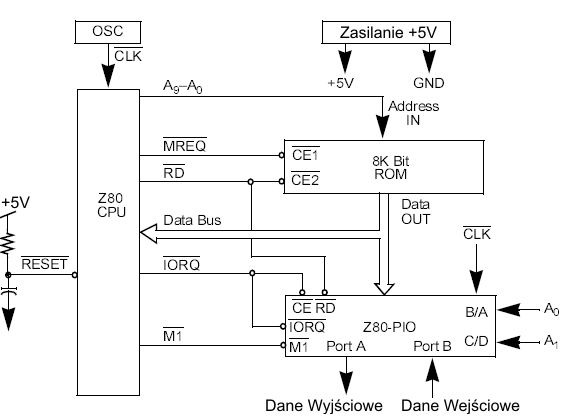
\includegraphics[width=0.6\textwidth]{z80minimalnySystemKomputerowy}
		\caption{Minimalny System Komputerowy Z80 \cite{eduinf}}
		\label{img:z80minimalnySystemKomputerowy}
	\end{figure}
		
	\section{z80emu-gui}
	Z80emu-gui to moduł zawierający interfejs użytkownika. Został napisany z pomocą biblioteki JavaFX. Projekt interfejsu uwzględnił stworzenie makiety w języku fxml zaprezentowanej na grafice \ref{img:z80Gui}. Większość interfejsów emulatorów posiada interfejs złożony z wielu okien, które można dowolnie zamykać i otwierać, a każde z nich zawiera osobny moduł. Dla przykładu, w Z80 simulator ide, edytor pamięci, asemblera lub manipulacja urządzeniami wejścia wyjścia zawarta jest w osobnych oknach. 
	W projekcie z80emu-gui postanowiono stworzyć interfejs zawierający wszystkie funkcje w jednym oknie. 
	
	\begin{figure}[h]
		\centering
		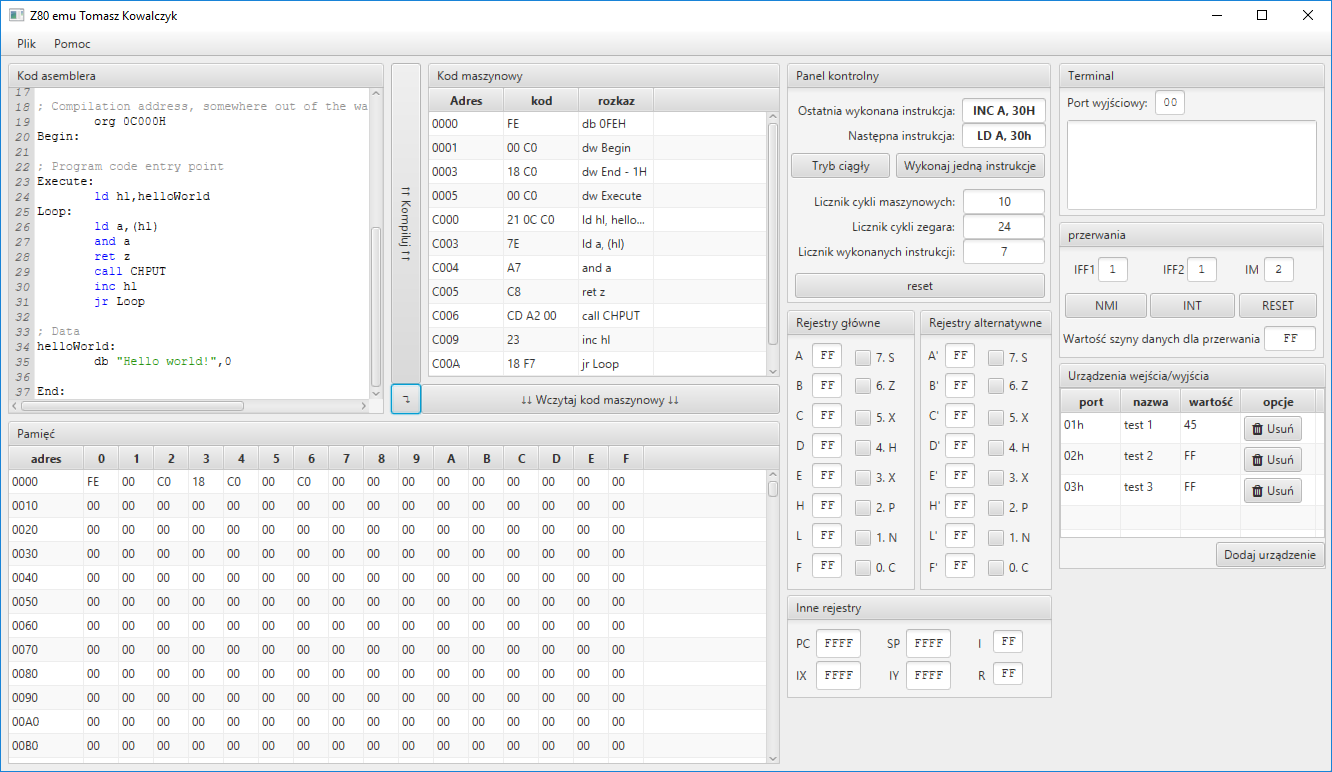
\includegraphics[width=1\textwidth]{z80Gui}
		\caption{Makieta interfejsu użytkownika}
		\label{img:z80Gui}
	\end{figure}
	 
	
	Elementy interfejsu podzielono na dwa mniejsze fragmenty w celu czytelniejszego wyjaśnienia. Część pierwsza zaprezentowana na grafice \ref{img:z80GuiPart1WithPoints} zawiera elementy związane z manipulacją pamięcią oraz kodem programu. Opis poszczególnych elementów umieszczonych na schemacie:
	\begin{enumerate}
		\item Edytor kodu asemblera, z prostym kolorowaniem składni.
		\item Widok kodu maszynowego w formie tabeli, zawierającej formacje o adresie rozkazu w pamięci, kodzie maszynowym oraz czytelnej dla człowieka nazwie instrukcji.
		\item Tabela reprezentująca moduł pamięci podłączony do procesora.
		\item Przycisk kompilujący kod asemblera (p. 1) do kodu maszynowego (p. 2).
		\item Przycisk wczytujący kod maszynowy programu(p. 2), do pamięci procesora (p. 3)
		\item Przycisk wykonujący kompilacje kodu asemblera (p. 1) a następnie wczytanie go do pamięci (p. 3).
	\end{enumerate}
	
	\begin{figure}[h]
		\centering
		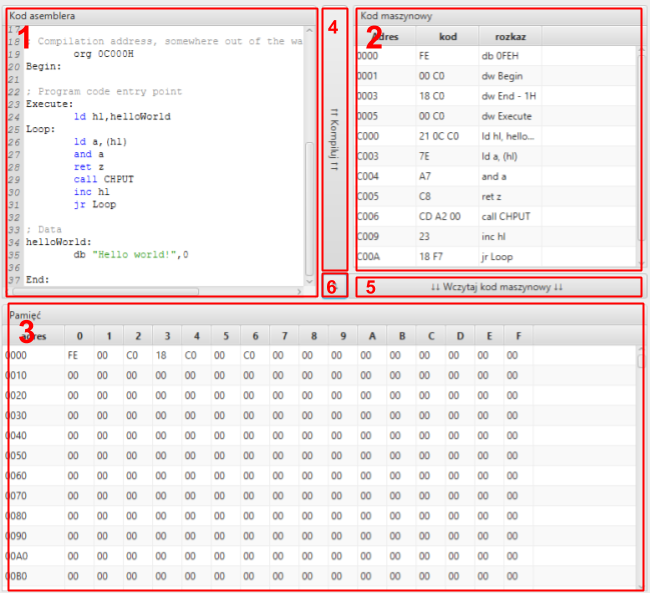
\includegraphics[width=1\textwidth]{z80GuiPart1WithPoints}
		\caption{Makieta interfejsu użytkownika z oznaczeniami. Część 1}
		\label{img:z80GuiPart1WithPoints}
	\end{figure}
	
	Drugą część interfejsu zaprezentowano na grafice \ref{img:z80GuiPart2WithPoints}. Poniżej opis poszczególnych elementów:
	\begin{enumerate}
		\item Główny panel kontrolujący proces emulacji, przedstawiający między innymi liczbę cykli maszynowych i zegara wykonywanego programu.
		\item Pola prezentujące nazwę ostatniej wykonanej i następnej w kolejce instrukcji procesora.
		\item Przycisk uruchamiający emulację ciągłą (ponownie jego wybranie zatrzymuje emulacje).
		\item Przycisk wykonujący pojedynczą, kolejną instrukcję procesora.
		\item Przycisk resetujący urządzenie.
		\item Widok rejestrów głównych i alternatywnych włącznie z flagami.
		\item Widok rejestrów I, R, PC, SP, IX, IY.
		\item Terminal wyjściowy, emulujący na stałe przypisane urządzenie. 
		\item Pole tekstowe z możliwością wpisania portu terminalu wyjściowego, pod jakim będzie przyjmował dane.
		\item Panel grupujący elementy interfejsu odpowiedzialne za przerwania.
		\item Przycisk wywołujący NMI (z ang. Non-Maskable Interrupt), sygnał przerwania niemaskowanego.
		\item Przycisk wywołujący INT (z ang. Interrupt), sygnał maskowanego przerwania.
		\item Przycisk wykonujący sygnał resetu.
		\item Pole tekstowe zawierające 8bitową wartość, jaką przyjmie szyna danych podczas przerwania.
		\item Tabela z listą podłączonych urządzeń wejścia/wyjścia.
		\item Przycisk pozwalający na usunięcie urządzenia wejścia/wyjścia.
		\item Przycisk dodający nowe urządzenie wejścia/wyjścia.
	\end{enumerate}
	
	\begin{figure}[h]
		\centering
		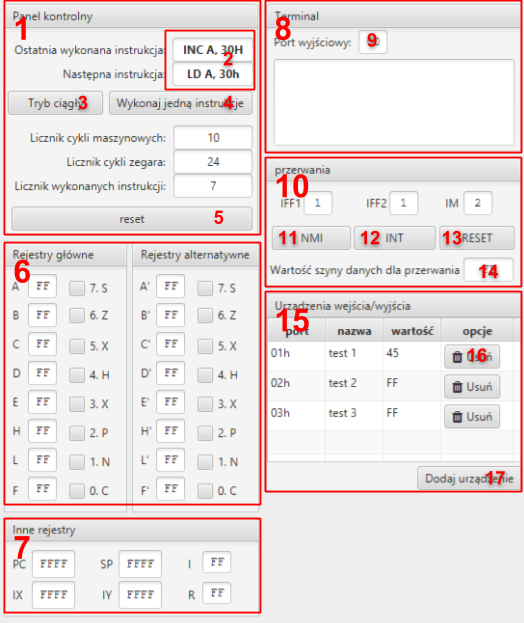
\includegraphics[width=0.8\textwidth]{z80GuiPart2WithPoints}
		\caption{Makieta interfejsu użytkownika z oznaczeniami. Część 2}
		\label{img:z80GuiPart2WithPoints}
	\end{figure}

	%tutaj o mvc
	
	